% ---------------------------------------------------------------------------- %
\subsection{Versuchsanordnung}
\label{subsec:versuchsanordnung}
% ---------------------------------------------------------------------------- %

Die       Versuchsanordnung      ist       schematisch      in       Abbildung
\ref{fig:versuchsapparaturSchema}     und    fotographisch     in    Abbildung
\ref{fig:versuchsapparaturFoto} dargestellt.

\begin{figure}[h!]
    \centering
    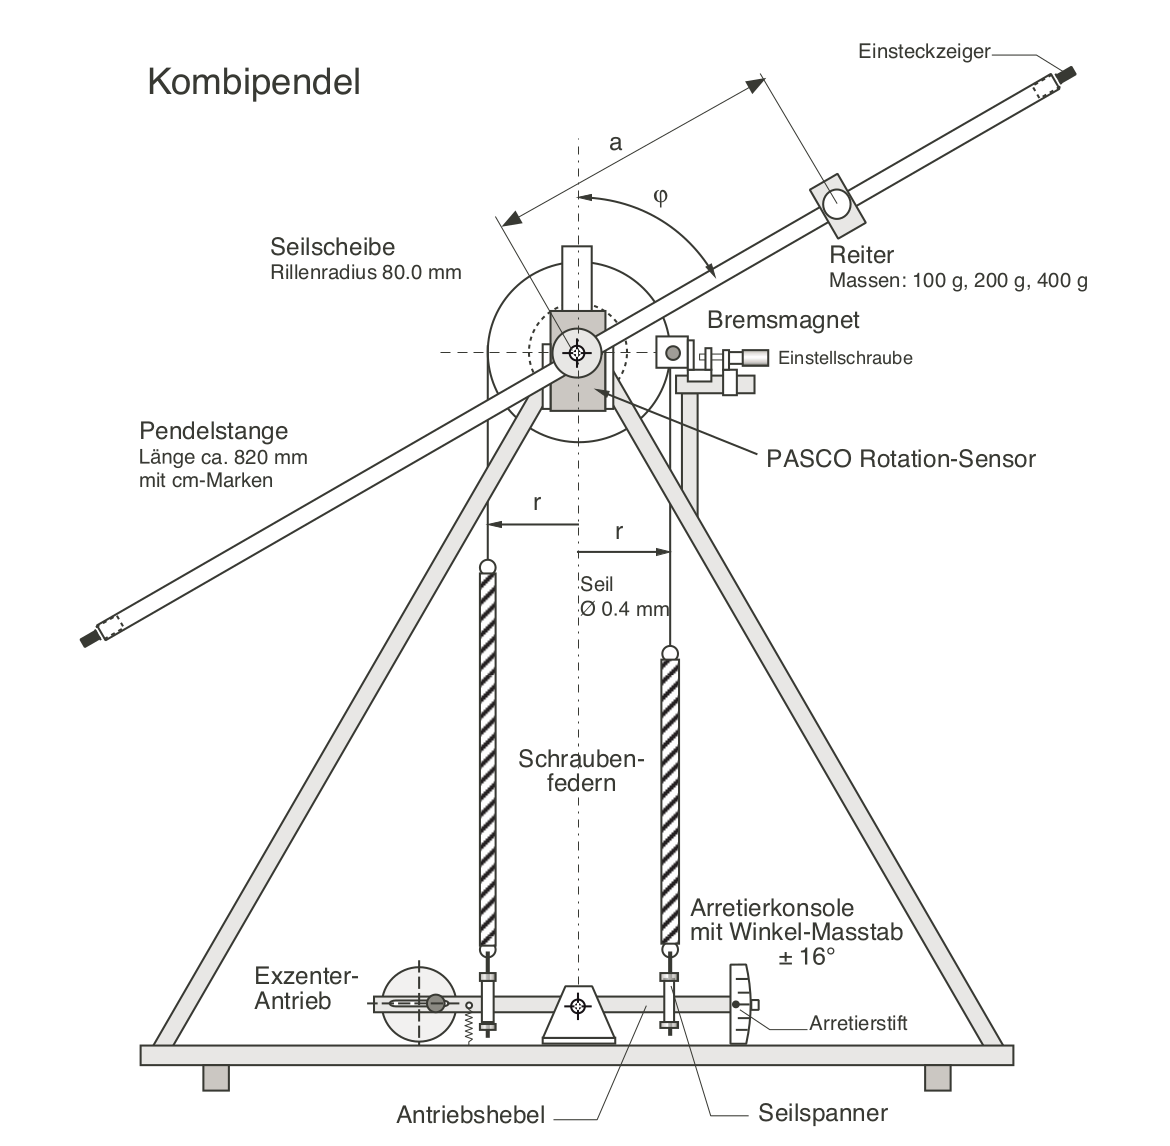
\includegraphics[width=.8\textwidth]{images/versuchsapparatur-schema.png}
    \caption{%
        Schematische Versuchsanordnung (Quelle: Versuchsanleitung)
    }
    \label{fig:versuchsapparaturSchema}
\end{figure}

\begin{figure}[h!]
    \centering
    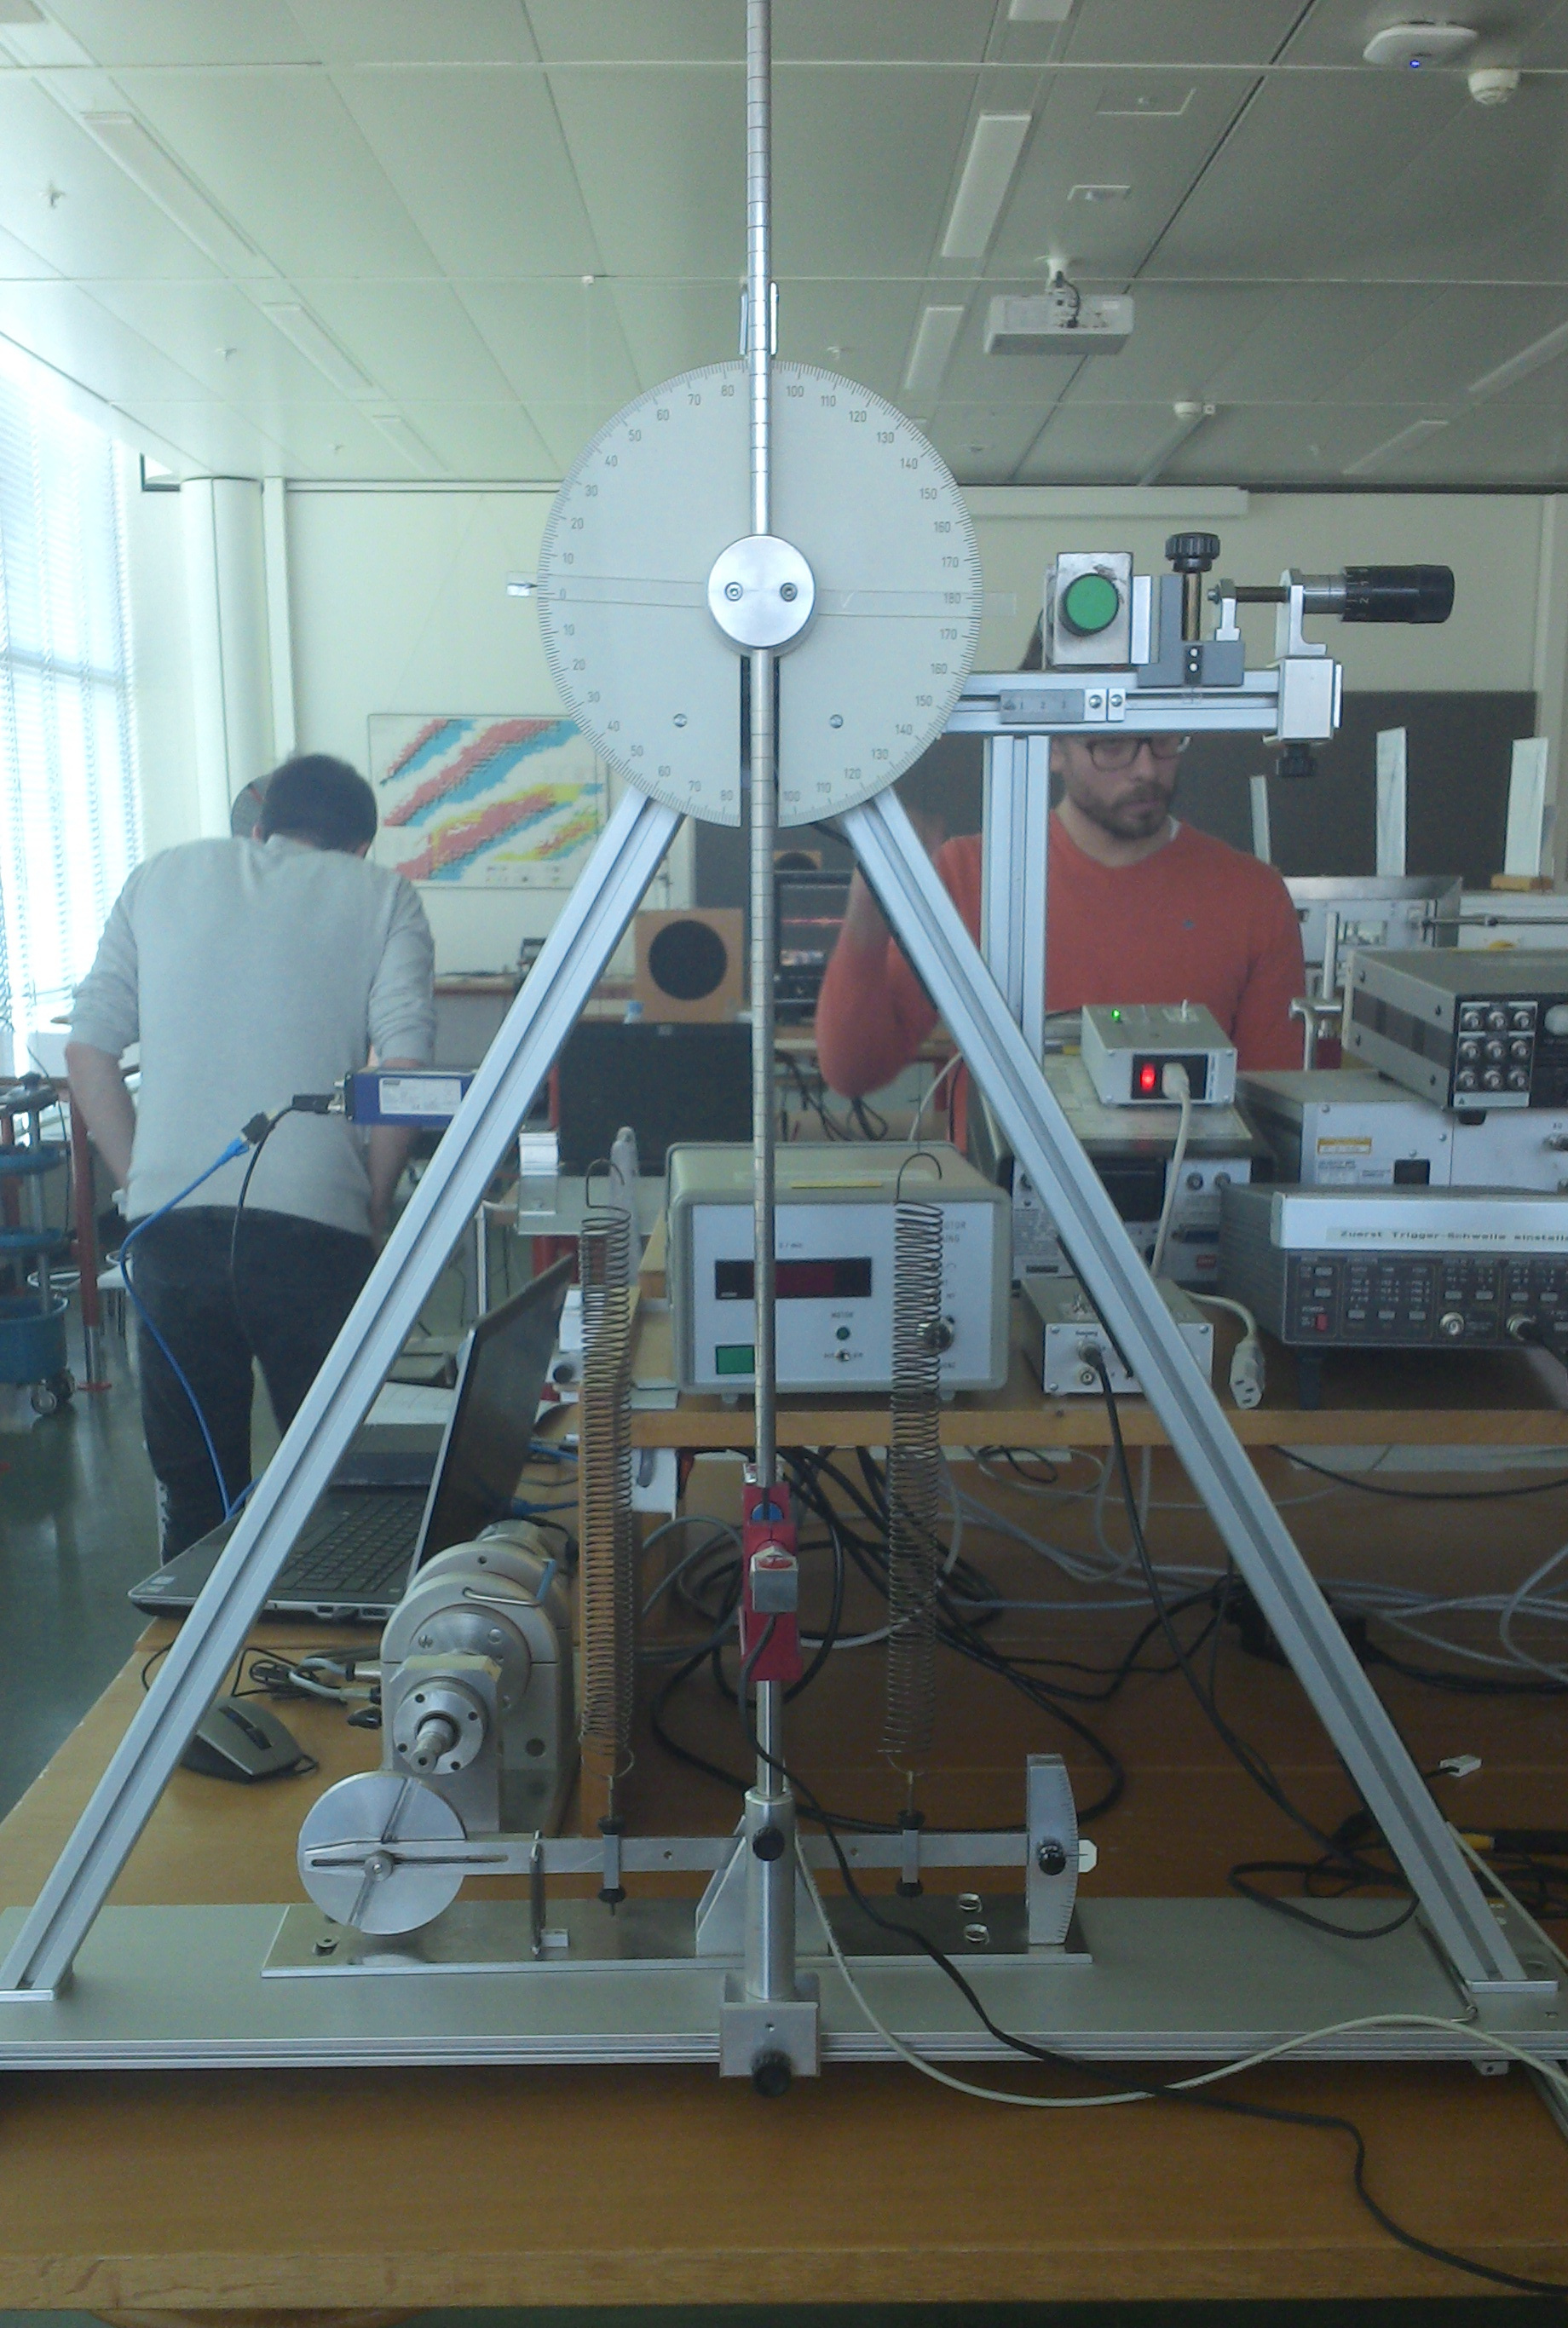
\includegraphics[width=.6\textwidth]{images/versuchsanordnung.jpg}
    \caption{%
        Versuchsanordnung im Labor
    }
    \label{fig:versuchsapparaturFoto}
\end{figure}

Die  Apparatur  besteht  aus  dreieckigem Rahmen,  welcher  eine  Pendelstange
lagert. Ein  Reiter (Zusatzgewicht)  kann  auf der  Pendelstange in  variablen
Abst\"anden montiert werden (beidseitig,  je nach gew\"unschter Konfiguration,
siehe Abschnitt zu theoretischen Grundlagen).

Es  ist auch  ein Bremsmagnet  und  ein Antrieb  f\"ur angeregte  Schwingungen
vorhanden, allerdings wurden diese bei unserem Versuch nicht benutzt.

Die  Schwingungen   der  Pendelstange   werden  mittels   einer  Lichtschranke
detektiert,  welche   variabel  positioniert   werden  kann,   abh\"angig  vom
durchgef\"uhrten   Versuch. Die  Lichtschranke   ist  an   eine  Auswertelogik
Marke  ``Eigenbau''  und  einen Frequenz\"ahler  der  Marke  <em>Keithley</em>
angeschlossen.

Wenn  ein bestimmter  Auslenk-Winkel  ben\"otigt wird,  kann  dieser an  einer
Winkelscheibe eingestellt werden.

% ---------------------------------------------------------------------------- %
\subsection{Ger\"ateliste}
\label{subsec:deviceList}
% ---------------------------------------------------------------------------- %

Die verwendeten Ger\"ate sind in Tabelle \ref{tab:deviceList} aufgef\"uhrt.

\captionof{table}{Hilfsmittel und Ger\"ateliste}
\label{tab:deviceList}
\begin{tabular}{ll}
    \toprule
    Ger\"at & Typ \\
    \midrule
    Frequenz-Z\"ahler                     & Keithley 776 Programmable Counter/Timer \\
    Lichtschranke und Auswerte-Elektronik & Lichtschranken-Logik 1 (Marke Eigenbau) \\
    Auswerteprogramm                      & QtiPlot \\
    \bottomrule
\end{tabular}


% ---------------------------------------------------------------------------- %
\subsection{Messvorgang/Messmethoden}
\label{subsec:measurementMethods}
% ---------------------------------------------------------------------------- %

Grunds\"atzlich  gab es  vier Arten  von Messungen:
\begin{itemize}
    \item
        Auslenkwinkel konstant, Reitermasse konstant, Reiterabstand variabel, Messung der Schwingungsperiode (Schwerependel, Kombipendel)
    \item
        Auslenkwinkel konstant, Reitermasse variabel, Reiterabstand konstant, Messung der Schwingungsperiode (Schwerependel, Kombipendel)
    \item
        Auslenkwinkel variabel, Reitermasse konstant, Reiterabstand konstant, Messung der Schwingungsperiode (Schwerependel, Kombipendel)
    \item
        Reitermasse konstant, Reiterabstand variabel, Messung des Winkels $\varphi_0$ der Ruhelage (Kombipendel invertiert, $a>a_{krit}$)
\end{itemize}

Abh\"angig davon, ob  die Apparatur als Schwerependel oder  als Kombipendel zu
betreiben war, wurden jeweils die Federn aus- bzw. eingeh\"angt.

% ---------------------------------------------------------------------------- %
\subsection{Proben/Versuchsobjekte}
\label{subsec:samples}
% ---------------------------------------------------------------------------- %

Es wurden Bronzefedern verwendet mit folgenden Daten gem\"ass Versuchsanleitung:
\begin{table}[h!]
    \centering
    \caption{Federn}
    \label{tab:springs}
    \begin{tabular}{lll}
        \toprule
        Typ, Material & Masse (kombiniert) & Federkonstante $k$ \\
        \midrule
        Bronzefedern (\SI{1.5}{\milli\meter} Durchmesser) & \SI{155.5}{\gram} & \SI{32.0}{\newton\per\meter} \\
        \bottomrule
    \end{tabular}
\end{table}

Die Federkonstante $k$ wurde in den  Versuchen mit dem Kombipendel jeweils als
Fit-Parameter verwendet und somit experimentell \"uberpr\"uft. Die Federn sind
\"uber ein Seil  des Durchmessers \SI{0.4}{\milli\meter} an  einem Seilrad mit
Rillendurchmesser \SI{160}{\milli\meter} mit der Apparatur verbunden (siehe auch
Schema der Apparatur).

Als Reiter standen verschiedene Massen zur Verf\"ugung, aufgelistet in Tabelle \ref{tab:riders}.

\begin{table}[h!]
    \centering
    \caption{Reiter}
    \label{tab:riders}
    \begin{tabular}{lll}
        \toprule
        Masse& Durchmesser  & L\"ange  \\
        \midrule
        \SI{100}{\gram} & \SI{30.2}{\milli\meter} & \SI{20}{\milli\meter} \\
        \SI{100}{\gram} & \SI{34.4}{\milli\meter} & \SI{15}{\milli\meter} \\
        \SI{200}{\gram} & \SI{34.4}{\milli\meter} & \SI{30}{\milli\meter} \\
        \SI{300}{\gram} & \SI{34.4}{\milli\meter} & \SI{45}{\milli\meter} \\
        \SI{400}{\gram} & \SI{34.4}{\milli\meter} & \SI{60}{\milli\meter} \\
        \bottomrule
    \end{tabular}
\end{table}

Bei  den Messungen  mit  Reitermassen \"uber  \SI{400}{\gram}  wurden aus  den
Reitern mit identischen Durchmessern jeweils ein Reiter zusammengesetzt. Dabei
wurde darauf  geachtet, dass der Schwerpunkt  der gesamten Reiterkonfiguration
seine Position auf der Stange nicht ver\"anderte.

% ---------------------------------------------------------------------------- %
%\subsection{Messungen}
%\label{subsec:measurements}
% ---------------------------------------------------------------------------- %
